\documentclass[10pt]{report}

\usepackage{amsmath}
\usepackage{amssymb}
\usepackage{graphicx}
\usepackage{helvet}

\setlength{\paperheight}{3in}
\setlength{\paperwidth}{4in}
\pdfpagewidth=\paperwidth
\pdfpageheight=\paperheight

\setlength{\textwidth}{3.75in}
\setlength{\textheight}{2.5in}

\setlength{\oddsidemargin}{-1.0in}
\setlength{\evensidemargin}{-1.0in}
\setlength{\topmargin}{-1.25in}

\newcommand{\sld}[1]{\newpage{\noindent\Large \ \ \ \underline{#1}}\vspace*{8pt}}
\newcommand{\spc}{\hspace*{0.25in}}

\newcounter{gmlrx}
\newcounter{gmlry}
\newcommand{\gmnode}[3]{\put(#1,#2){\circle{20}}\put(#1,#2){\makebox(0,0){$#3$}}}
\newcommand{\gmplate}[5]{
\setcounter{gmlrx}{#1}\addtocounter{gmlrx}{#3}
\setcounter{gmlry}{#2}\addtocounter{gmlry}{-#4}
\put(#1,#2){\line(1,0){#3}}
\put(#1,#2){\line(0,-1){#4}}
\put(\value{gmlrx},\value{gmlry}){\line(-1,0){#3}}
\put(\value{gmlrx},\value{gmlry}){\line(0,1){#4}}
\setcounter{gmlrx}{#1}\addtocounter{gmlrx}{5}
\setcounter{gmlry}{#2}\addtocounter{gmlry}{-6}
\put(\value{gmlrx},\value{gmlry}){\makebox(0,0){$#5$}}
}

\newcommand{\mypart}[1]{\newpage\vspace*{36pt}\noindent \spc{\huge #1}}


\begin{document}
\sf%
\vspace*{12pt}
\noindent
\spc{\huge Models of Data Annotation}
\\[8pt]
\spc{\huge  and Probabilistic Corpora}
\\[24pt]
\spc{\Large Bob Carpenter} 
\\[12pt]
\spc{\itshape Columbia Uni. \ \& \ LingPipe, Inc.}
\\[24pt]
\mbox{ } \hfill \spc {\footnotesize CMU Reunion}


\mypart{Modeling Corpus Annotation}


\sld{Motivation: Estimate Useful Quantities}

\vspace*{-4pt}
\begin{itemize}
\item Label for item
\item Prevalence of item labels
\item Accuracy/bias of each annotator (adjust ``votes'')
\item Mean annotator accuracy and bias
\item Annotator variability
\begin{itemize}
\footnotesize
\item Use these instead of $\kappa$ stats to evaluate coding standard
\end{itemize}
\item Predict effect of new annotation 
\hfill
\item All with Bayesian probability estimates of uncertainty
\end{itemize}


\sld{(Mostly) Generative Model Sketch}

\begin{itemize}
\item $\pi \ |\ $ \ \hfill item prevalence
\item $z_i \  | \ \pi$ \ \hfill true category for item $i$
\\
\item $\theta_j \ | \ $ \ \hfill response for annotator $j$ 
\\
\item $y_{i,j} \ | \ z_i,\ \theta_j$ \ \hfill label by annotator $j$ for item $i$
\end{itemize}
\vfill
\spc{\small (Dawid and Skene 1979)}


\sld{Fully Generative Model Sketch}

\vspace*{-4pt}
\begin{itemize}
\item $\alpha$  \hfill (constant) item prevalence prior
\item $\pi \ | \ \alpha$ \hfill item prevalence
\item $z_i \  | \ \pi$ \hfill true category for item $i$
\\[-6pt]
\item $\beta$ \hfill (constant) annotator response prior
\item $\theta_j \ | \ \beta$ \hfill response for annotator $j$ 
\\[-6pt]
\item $y_{i,j} \ | \ z_{i},\ \theta_{j}$ \hfill label by annotator $j$ for item $i$
\end{itemize}



\sld{Hierarchical Model Sketch}

\vspace*{-6pt}
\begin{itemize}
\item $\alpha_0$ \hfill (constant) item prevalence hyperprior
\item $\alpha \ | \ \alpha_0$  \hfill item prevalence prior
\item $\pi \ | \ \alpha$ \hfill item prevalence
\item $z_i \  | \ \pi$ \hfill true category for item $i$
\\[-6pt]
\item $\beta_0$ \hfill (constant) annotator response hyperprior
\item $\beta \ | \ \beta_0$ \hfill annotator response prior
\item $\theta_j \ | \ \beta$ \hfill response for annotator $j$ 
\\[-6pt]
\item $y_{i,j} \ | \ z_{i},\ \theta_{j}$ \hfill label by annotator $j$ for item $i$
\end{itemize}

\sld{Estimation}

\begin{itemize}
\item MLE or MAP Point Estimates
\begin{itemize}
\footnotesize
\item count with gold labels $z_i$ \hfill (Snow et al. 2009)
\item EM w/o gold labels \hfill (Dawid and Skene 1979)
\item EM semi-supervised \hfill (Tang and Lease 2011)
\item Hierarchical case degenerates to 0 variance
\end{itemize}
\item Full Bayesian Posterior
\begin{itemize}
\footnotesize
\item Gibbs sampling w/o gold labels \hfill (Carpenter 2008)
\item Gibbs sampling semi-supervised \hfill (Carpenter 2011)
\item Full Bayes: Estimation uncertainty used in inference
\item Handles hierarchical case
\end{itemize}
\end{itemize}


\mypart{Discussion Points}

\sld{Is the Truth Out There?}

\begin{itemize}
\item Existing corpora are not 24-carat gold
\item But is the truth even out there?
\begin{itemize}
\footnotesize
\item Given the evolving and creative nature of language, 
coding standards are always vague and ambiguous
\item Graded class membership gives vagueness (e.g., ordinal sentiment
or modality)
\item Items act like two classes (e.g., POS tagging, NE, word sense)
\item Author/speaker may not have been clear
\end{itemize}
\end{itemize}



\sld{Item Difficulty and Random Effects}

\begin{itemize}
\item Clear some items are harder to annotate than others
\item Could add an item difficulty parameter
\item Difficult to estimate with few annotators/item
\item Use features of annotators (e.g., skill
level, specialty, native language, age, sex, \ldots)
\item Use features of items annotated (e.g., source,
length, language, difficulty of language, \ldots)
or items being annotated
\item Can help with active learning, but not necessary
\end{itemize}


\sld{Adding System as Another Annotator}

\begin{itemize}
\item Assume item content (e.g., text) is available
\item Assume trainability of probability model for task
\item Throw model in as another annotator
\item Estimate (train) everything jointly
\vfill
(Raykar et al. 2010)
\end{itemize}


\sld{Probabilistic Training and Testing}

\begin{itemize}
\item Treat ``truth'' as uncertain (i.e., measurement error)
\item Model provides probability estimates of different labels
\item Easy to train probabilisitic models with probabilistic ``truth'' 
(e.g, HMMs, CRFs, naive Bayes, logistic regression, \ldots)
\item Model then tracks uncertainty in gold standard
\item Evaluate with expected square error or log loss
\end{itemize}

\sld{E.g., Probabilistic Binary Classification}

\vspace*{-6pt}
\begin{itemize}
\item Probabilistic truth: $y \in [0,1]$ \  (discrete special case)
\item Prediction: $\hat{y} \in [0,1]$
\item Log Loss: ${\mathcal L}(y,\hat{y}) = - \log (y \times \hat{y} \
+ \
(1 - y) \times (1 - \hat{y}))$
\item Minimum Error Prediction:  $y = \arg\min_{\hat{y}} \ {\mathcal L}(y,\hat{y})$
\item Predictors: $x \in \mathbb{R}^D$ \ \ Coefficients: $\beta \in \mathbb{R}^D$
\item Logistic Regression MLE
\\[6pt]
 $\beta^{*} =
  \arg\min_{\beta} \ {\mathcal L}(y,\mbox{logit}^{-1}(\beta^T x))$
\hfill (convex, so exists)
\item Pushes prediction for $x$ to $y$, reducing overconfidence
\end{itemize}


\mypart{The End, or \ldots}

\mypart{What's wrong with $\kappa$}

\sld{{\Huge $\kappa$} is ``Chance-Adjusted Agreement''}

$\kappa(A,E) = {\displaystyle\frac{A - E}{1 - E}}$

\begin{itemize}
\item $A$ is agreeement rate 
\item $E$ is chance agreement rate
\end{itemize}
\vspace*{8pt}
\begin{itemize}
\item Industry standard
\item Attempts to adjust for difficulty of task
\item $\kappa$ above arbitrary threshold considered ``good''
\end{itemize}


\sld{Problems with {\Huge $\kappa$}}

\begin{itemize}
\item $\kappa$ intrinsically a pairwise measure
\item $\kappa$ only works for subset of shared annotations
\item Not used in inference after calculation
\begin{itemize}
\footnotesize
\item $\kappa$ doesn't predict corpus accuracy 
\item $\kappa$ doesn't predict annotator accuracy 
\end{itemize}
\item $\kappa$ reduces to agreement for hard problems
\begin{itemize}
\item {\large $\lim_{E \rightarrow 0} \kappa(A,E) = A$}
\end{itemize}
\end{itemize}


\sld{Problems with {\Huge $\kappa$} (cont)}

\begin{itemize}
\item $\kappa$ assumes annotators all have same accuracies
\item $\kappa$ assumes annotators are unbiased 
\begin{itemize}
\footnotesize
\item if biased in same way, $\kappa$ too high
\end{itemize}
\item $\kappa$ assumes 0/1 items same value
\begin{itemize}
\footnotesize
\item common: low prevalence, high negative agreement
\end{itemize}
\item $\kappa$ typically estimated without variance component
\item $\kappa$ assumes annotations for an item are uncorrelated
\begin{itemize}
\footnotesize
\item items have correlated errors, $\kappa$ too high
\end{itemize}
\end{itemize}





\mypart{Mechanical Turk Examples}
\vfill
(Carpenter, Jamison and Baldwin, 2008)


\sld{Case 1: Named Entities}

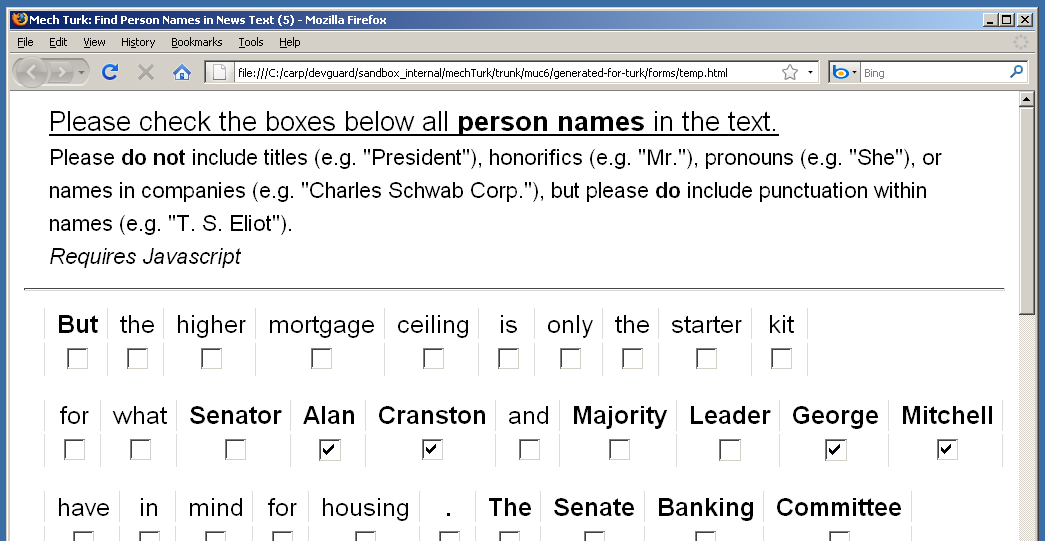
\includegraphics[width=0.95\textwidth]{pngs/big-ne-form.png}


\sld{Named Entities Worked}

\begin{itemize}
\item Conveying the coding standard
\begin{itemize}
\footnotesize
\item official MUC-6 standard dozens of pages
\item examples are key
\end{itemize}

\item Fitts's Law
\begin{itemize}
\footnotesize
\item time to position cursor inversely proportional to target size
\item highlighting text: fine position + drag + position
\item pulldown menus for type: position + pulldown + select
\item checkboxes for entity at a time: fat target click
\end{itemize}
\end{itemize}

\sld{Discussion: Named Entities}

\vspace*{-6pt}
\begin{itemize}
\item 190K tokens, 64K capitalized, 4K person name tokens
\begin{itemize}
\footnotesize
\item 4K / 190K = 2.1\% prevalence of entity tokens
\end{itemize}
\item 10 annotators per token
\item 100+ annotators, varying numbers of annotations
\item Less than a week at 2 cents/400 tokens (US\$95)
\item Aggregated Turkers better than LDC data
\begin{itemize}
\footnotesize
\item Correctly Rejected:
{\tt\footnotesize Webster's, Seagram, Du Pont,
\\
Buick-Cadillac, Moon, erstwhile Phineas Foggs}
\item Incorrectly Accepted: {\tt\footnotesize Tass}
\item Missed Punctuation: {\tt\footnotesize J~E.~``Buster'' Brown}
\end{itemize}

\end{itemize}




\sld{Case 2: Morphological Stemming}

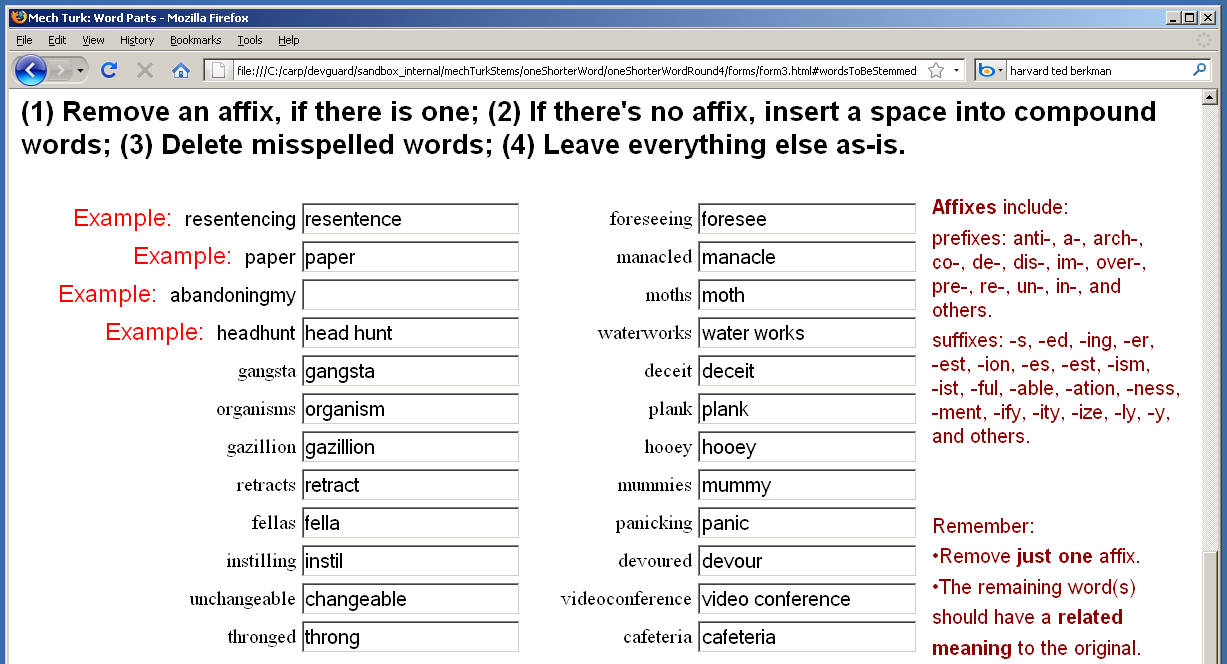
\includegraphics[width=0.95\textwidth]{pngs/stems-v4.png}

\sld{Morphological Stemming Worked}

\begin{itemize}
\vspace*{-8pt}
\item Coded and tested by intern (Emily Jamison of OSU)
\begin{itemize}
\footnotesize
\item Less than one month to code, modify and collect 
\end{itemize}
\item Three iterations of coding standard, Four of instructions
\begin{itemize}
\footnotesize
\item began with full morphological segmentation (too hard)
\item simplified task to one stem with full base (more ``natural'')
\item added previously confusing examples and sample affixes
\end{itemize}

\item Added qualifying test

\item 60K (50K frequent Gigaword, 10K random) tokens
\item 5 annotators / token
\end{itemize}



\end{document}
